\documentclass[10pt]{article}
\usepackage{lipsum}
\usepackage{indentfirst}
\usepackage[portuguese]{babel}
\usepackage{graphicx}
\usepackage[a4paper,left=2cm,right=2cm,top=2cm,bottom=2cm]{geometry}

\linespread{1.5}
\begin{document}
	

\title{\uppercase{\textbf{Relatório: Movimento Harmônico Amortecido}}}
\author{Saulo Ferreira de Souza 83339 \protect\\ Rodrigo Otavio de Lima 89386}
\maketitle

\setlength{\parindent}{2cm}

\section{OBJETIVOS}

Detalhar as metodologias e procedimentos utilizados no experimento do movimento harmônico amortecido, utilizando gráficos e tabelas como ferramentas auxiliares.

\section{INTRODUÇÃO}

Na natureza há um grande número de processos que se repetem em intervalos de tempo iguais. Estes são os chamados fenômenos periódicos, entre os quais podem ser citados o movimento de um pêndulo, a oscilação de um massa suspensa em uma mola e a vibração de uma corda. Embora se diferenciem, as naturezas destas oscilações são bastante análogas as formulações matemáticas utilizadas para descrevê-las. Uma grandeza física fundamental para a análise de todos esses fenômenos é o período $T$, definido como o tempo correspondente a uma oscilação completa.

\section{METODOLOGIA}

\subsection{MATERIAL UTILIZADO}

Barbante, uma massa de 100 g, cronômetro e trena milimetrada, regra milimetrada, papel milimetrado e papel monolog.

\subsection{PROCEDIMENTO}

A massa de 100 g foi amarrada na extremidade de um barbante com $L = (1,90 \pm 0,05)$ m de comprimento, fixado no teto, de tal forma que esse pêndulo simples oscilasse num plano vertical. Uma régua milimetrada foi posicionada nesse plano, utilizada como referência para a posição do pêndulo, de forma que o ponto 0 da régua representasse a posição de equilíbrio. A Figura \ref{fig:pendulo} representa o esquema do experimento.

\begin{figure}
	\begin{center}
		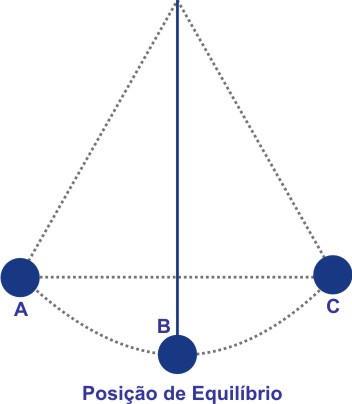
\includegraphics{desenho1-1.jpg}
		\caption{Esquema do experimento}
		\label{fig:pendulo}
	\end{center}

	
\end{figure}

\subsubsection{Primeiro experimento}
Na primeira parte do experimento, o pêndulo foi deslocado 33 cm em relação a régua milimetrada, formando um ângulo de $10^{\circ}$ com a vertical, e abandonado dessa posição. Para determinar o período médio desse pêndulo ($T_{medio}$), foi medido o tempo correspondente a 10 oscilações completas com a utilização do cronômetro, repetindo esse procedimento 3 vezes, obtendo a média dos tempos medidos. A média dos 3 resultados determinou $T_{medio}$.

Em seguida, foi calculado o período teórico ($T_{teorico}$) utilizando a Equação (\ref{eq:periodo}), e comparado com o $T_{medio}$ encontrado no experimento. O valor adotado para a gravidade foi $g = (9,78 \pm 0,01) m/s^2$. A Equação (\ref{eq:derivada}) foi utilizada para encontrar o desvio do resultado teórico. 

\begin{equation}
T_{teorico} = 2\pi\sqrt \frac{L}{g}
\label{eq:periodo}
\end{equation}

\begin{equation}
\Delta T_{teorico} = \frac{\partial T_{teorico}}{\partial L}\Delta t + \frac{\partial T_{teorico}}{\partial g}
\label{eq:derivada}\Delta g
\end{equation}

\subsubsection{Segundo experimento}

O pêndulo foi afastado de uma distância horizontal de aproximadamente 55 cm em relação à posição inicial e abandonado. O tempo necessário para que o pêndulo alcançasse as amplitudes 50, 45, 40, 35, 30, 25 e 20 centímetros foi marcado utilizando o cronômetro. Este procedimento foi repedido 3 vezes, e no final foi calculada a média entre os tempos de cada posição para definir o tempo médio. A amplitude em relação ao tempo é dada pela Equação (\ref{eq:amplitude}), onde $\alpha = b/2m$.

\begin{equation}
A(t) = A_0e^{-\alpha t}
\label{eq:amplitude}
\end{equation}

\section{RESULTADOS}

\subsection{Primeiro experimento}
A Tabela \ref{tab:table1} exibe os resultados do primeiro experimento. As 3 primeiras colunas representam o tempo médio obtido das 10 oscilações em cada repetição. A última coluna representa a média dos 3 resultados. 

\begin{table}[h!]
	\begin{center}
		\begin{tabular}{|c|c|c|c|}
			\hline
			$T_1$ & $T_2$ & $T_3$ & $T_{medio}$ \\
			\hline
			$(2,76 \pm 0,05)s$ & $(2,77 \pm 0,05)s$ & $(2,76 \pm 0,05)s$ & $(2,77 \pm 0,05)s$\\
			\hline			
		\end{tabular}
		\caption{Média obtida em cada tentativa e tempo médio obtido no experimento}
		\label{tab:table1}
	\end{center}
\end{table}

O valores $T_{teorico}$ e $\Delta T_{teorico}$ foram calculados substituindo os valores de $L$ e $g$ e seus respectivos erros nas equações (\ref{eq:periodo}) e (\ref{eq:derivada}), respectivamente. 

\begin{equation}
	T_{teorico} = 2\pi\sqrt\frac{1,90m}{9,78m/s^2} = 2,77s
\end{equation}

\begin{equation}
\Delta T_{teorico} = \frac{\pi}{\sqrt{ 1,90\times9,78}}\times 0,05 - \pi \sqrt{ \frac{1,90}{9,78^3}} \times 0,01 = 0,04
\end{equation}

É possível notar que o período encontrado no experimento ficou muito próximo do valor teórico, devido ao fato de que foi escolhido um ângulo pequeno ($10^\circ$) no experimento, de forma que os termos senoidais que multiplicam a equação (\ref{eq:periodo}) ficam muito pequenos, podendo ser desconsiderados.

\subsection{Segundo experimento}
O resultado médio encontrado no segundo experimento em cada amplitude esta representado na Tabela \ref{tab:table2}

\begin{table}[ht]
	\begin{center}
		\resizebox{\textwidth}{!}{			\begin{tabular}{|c|c|c|c|c|c|c|c|c|}
			\hline
			A & 50 cm & 45 cm & 40 cm & 35 cm & 30 cm & 25 cm & 20 cm \\
			\hline
			$t+\Delta t$ & $(20,44 \pm 0,05)s$ & $(47,42 \pm 0,05)s$ & $(82,89 \pm 0,05)s$ & $(122,85 \pm 0,05)s$ & $(172,19 \pm 0,05)s$ & $(234,46 \pm 0,05)s$  & $(320,82 \pm 0,05)s$\\
			\hline			
		\end{tabular}}
		\caption{Tempo médio em cada amplitude}
		\label{tab:table2}
	\end{center}
\end{table}

O gráfico da amplitude em função do tempo foi desenhado em um papel milimetrado. As devidas proporções foram calculadas, de forma que o gráfico ocupasse todo o espeço disponível. O gráfico se aproximou de uma função exponencial, ficando de acordo com a equação (\ref{eq:amplitude}).

Para encontrar os valores e $A_0$ e $\alpha$, a equação (\ref{eq:amplitude}) foi linearizada, resultando na equação (\ref{eq:linear}). A aplicação das amplitudes nessa equação deu origem à Tabela \ref{tab:table3}.

\begin{equation}
\ln(A) = \ln({A_0e^{-\alpha t}})
\label{eq:linear}
\end{equation}

\begin{table}[ht]
	\begin{center}
		\resizebox{\textwidth}{!}{			\begin{tabular}{|c|c|c|c|c|c|c|c|c|}
				\hline
				$ln A$ & 3,91 cm & 3,81 cm & 3,69cm & 3,55 cm & 3,40 cm & 3,22 cm & 2,99 cm \\
				\hline
				$t+\Delta t$ & $(20,44 \pm 0,05)s$ & $(47,42 \pm 0,05)s$ & $(82,89 \pm 0,05)s$ & $(122,85 \pm 0,05)s$ & $(172,19 \pm 0,05)s$ & $(234,46 \pm 0,05)s$  & $(320,82 \pm 0,05)s$\\
				\hline			
		\end{tabular}}
		\caption{Amplitudes após a linearização, com seus respectivos tempos médios}
		\label{tab:table3}
	\end{center}
\end{table}

Os pontos da Tabela \ref{tab:table3} foram desenhados em um papel milimetrado, e a melhor reta foi traçada. Com essa reta, foi encontrado o valor $A_0 = (3,94 \pm 0,05) cm$, onde ocorre a interseção da reta com o eixo $y$. O valor de $\alpha$ foi encontrado aplicando a equação (\ref{eq:inclinacao}).

\begin{equation}
\alpha = \frac{\Delta y}{\Delta x} = \frac{(3,0622 - 3,1705) cm}{(285,12-249,48)s} = -0,00304cm/s
\label{eq:inclinacao}
\end{equation}

Além disso, os pontos da Tabela \ref{tab:table3} foram desenhados em um papel monolog, e a melhor reta foi traçada. Com essa reta, foi encontrado o valor $A_0 = (1,680 \pm 0,05) cm$, onde ocorre a interseção da reta com o eixo $y$. O valor de $\alpha$ foi encontrado aplicando a equação (\ref{eq:inclinacao}).

\begin{equation}
\alpha = \frac{\Delta y}{\Delta x} = \frac{(0,40 - 1,6) cm}{(214,55-64,365)s} = -0,00799cm/s
\label{eq:inclinacao}
\end{equation}

\section{CONCLUSÃO}

Os resultados encontrados nos experimentos foram de acordo com o esperado pela formulação teórica, com pequenos desvios aceitáveis. É possível notar que o sucesso do experimento em aproximar dos valores teóricos, foi devido à suas repetições, confirmando a evidência de quanto mais se repete os testes experimentais, mais a média dos resultados observados converge para o valor esperado.  

\begin{thebibliography}{9}
	
	\bibitem{lamport94}
	"PRATICA: MOVIMENTO HARMÔNICO AMORTECIDO."
	\textit{Departamento de Física, UFV.}


\bibitem{lamport94}
Young and Freeeman.
\textit{FÍSICA II - Termodinâmica e Ótica.}	
\end{thebibliography}

\end{document}

